\documentclass[10pt,letterpaper]{article}
\usepackage{amsmath}
\usepackage{amssymb}
\usepackage{fancyhdr}
\usepackage[bottom=1in, top=1in, left=1in, right=1in]{geometry}
\usepackage{graphicx}
\usepackage{here}
\usepackage{subfigure}
\usepackage[T1]{fontenc}
\DeclareGraphicsExtensions{.pdf,.png,.jpg}

\pagestyle{fancy}
\setlength{\headheight}{.5in}
\setlength{\parindent}{0in}

\begin{document}

\rhead{
          Paul Boschert\\
          10/22/2015\\
          CSCI 5229 - Computer Graphics: Project Proposal \\
      }

\textbf{\textit{Summary:}} I propose to create a software package to render measurements from a fiber interrogation system.
\\
\\
\textbf{\textit{Problem Statement:}} State of the art fiber interrogation systems only have the ability to interrogate < 100 sensors.  With our unique laser, we have the ability to measure over 1300 sensors.  Collecting this much data and displaying it efficiently for our unique laser is difficult.  There are applications and libraries available to use, but none of these are sufficiently complete, or they do not support using a GPU to render the data.
\\
\\
\textbf{\textit{Project Goals:}}
\begin{enumerate}
  \item Waterfall plot.  An example using gnuplot which uses the CPU to render the plot is in Figure \ref{fig:waterfallPlot}.
    \begin{figure}[h]
      \centering
      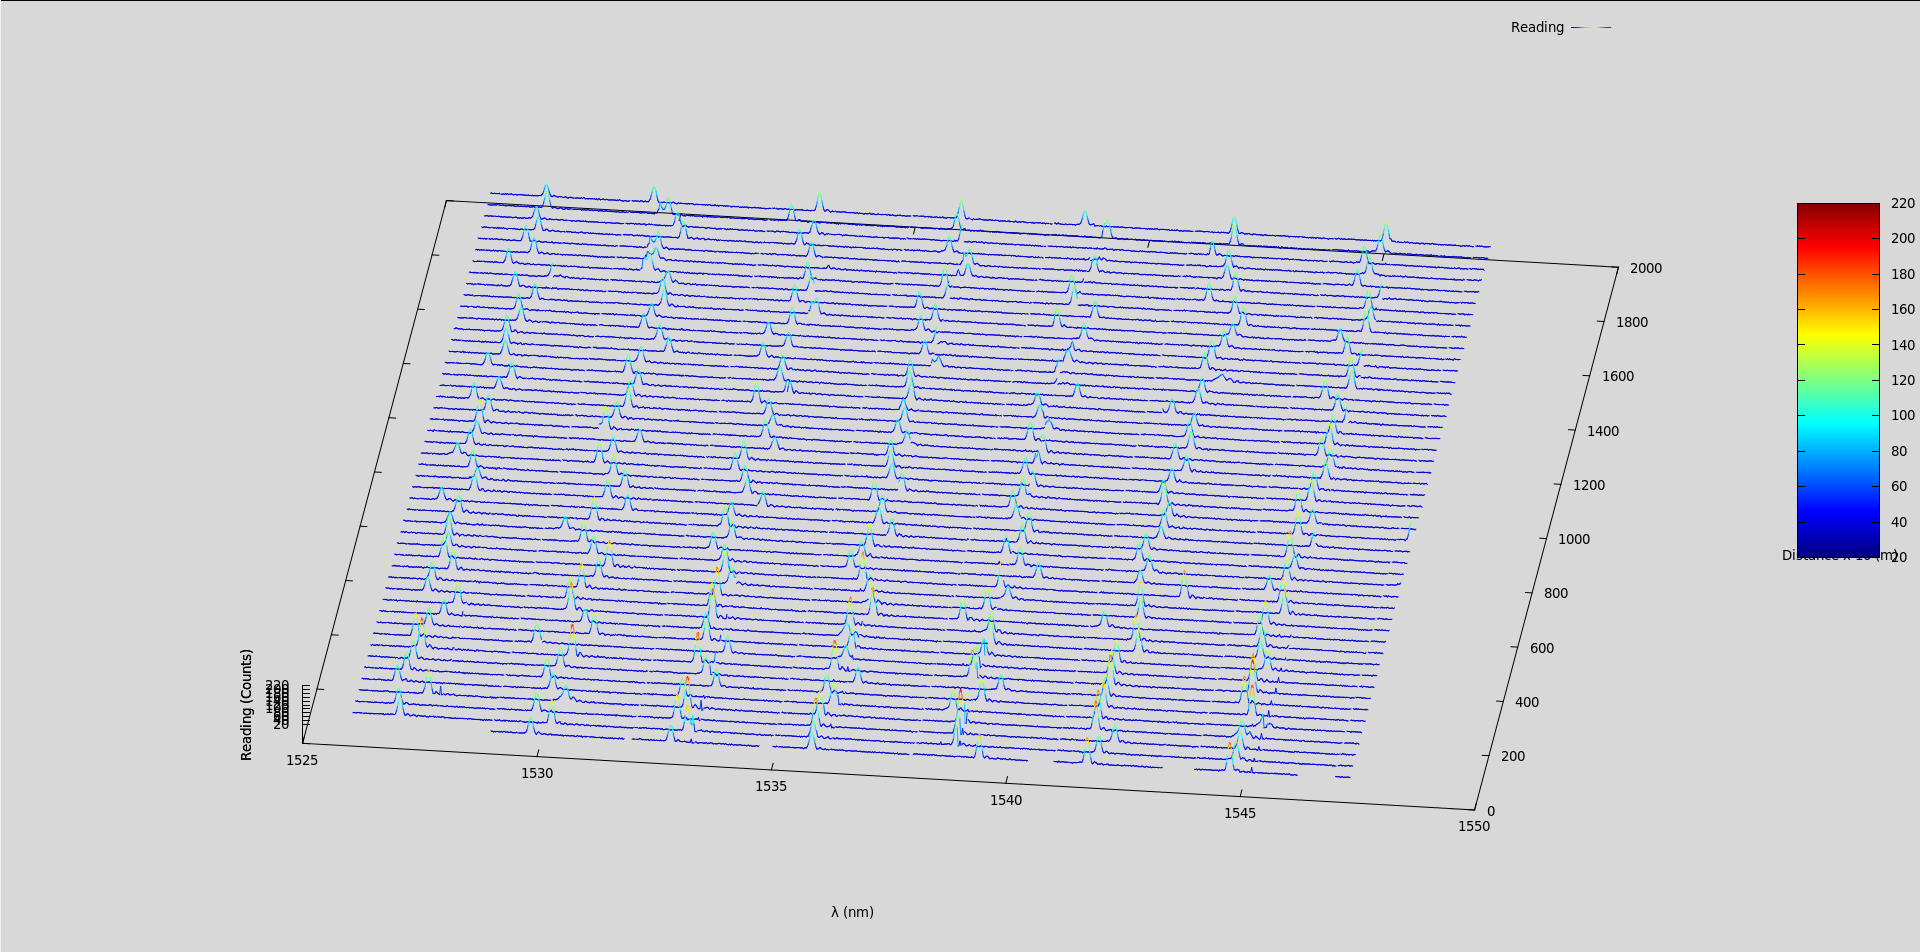
\includegraphics[scale=.25]{waterfallPlot}
      \caption{Waterfall plot}
      \label{fig:waterfallPlot}
    \end{figure}
    \\
    In addition to simply displaying the plot.  It will be interactive, allowing the user to zoom in on a specific reflection peak, change the plotting color scheme, change the connecting lines (lines, points, or lines with points).
  \item Display 1300 sensors.  The idea here is to have a scrolling plot of each sensor.  The user is able to select one of these sensors, and the selected plot will enlarge so the user can see more details about the sensor.
  \item Raw data plot.  Show the raw data and allow the user to zoom in on any section.  An example using pyqtgraph which uses the CPU to render the plot is in Figure \ref{fig:rawAcquisitionPlot}.
    \begin{figure}[h]
      \centering
      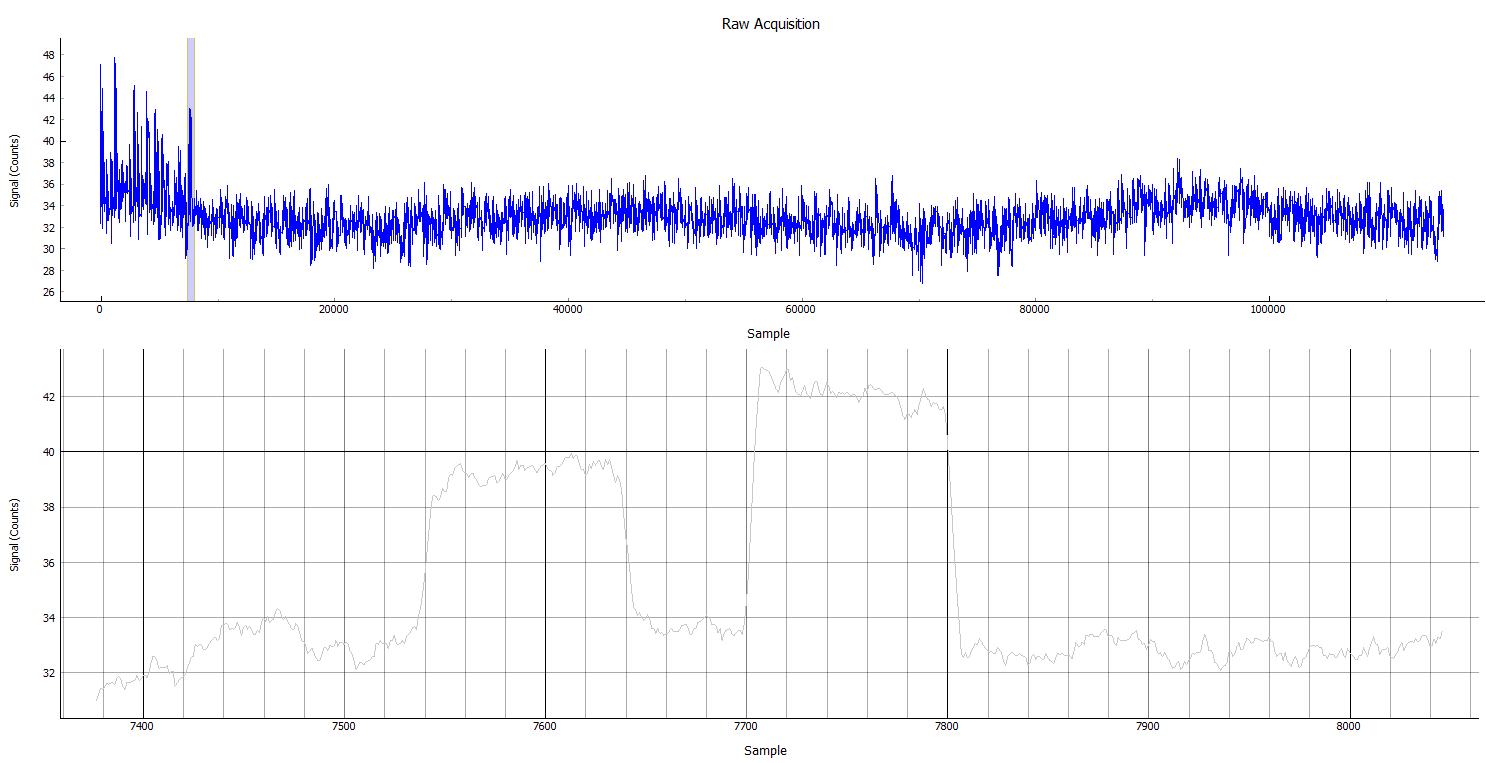
\includegraphics[scale=.42]{rawAcquisitionPlot}
      \caption{Raw Acquisition Plot}
      \label{fig:rawAcquisitionPlot}
    \end{figure}
  \item Peak tracking plot(s).  To show the stability of our laser, we can track the peak of the sensor reflection over time.
\end{enumerate}

\end{document}
